\section{单组分体系}


\begin{frame}
    \frametitle{单组分体系}

    \large 对于单组分体系$C=1$
    
    \begin{itemize}
        \item[\bullet] 根据相律$f=C-P+2=3-P$，说明单组分体系中最多三相共存，此时体系没有独立变量。
        \item[\bullet] 当$P=1$时$f=2$，即体系为双变量体系，指温度和压力在一定范围内可任意变动。
        \item[\bullet] 当$P=2$时$f=1$，此时温度和压力两个变量存在一定的依存关系，指定了一个，另一个也随之确定下来。
    \end{itemize}

\end{frame}


\begin{frame}
    \frametitle{相变时体系的压力随温度的变化关系}

    \large 定温定压下，某纯物质两相平衡共存，根据相平衡条件，即有
    $$\mu^{\alpha}(T, p)=\mu^{\beta}(T, p)$$
    当温度改变d$T$，压力改变d$p$后，达到新的平衡状态，即
    $$\mu^{\alpha} + \mathrm{d}\mu^{\alpha} =\mu^{\beta} + \mathrm{d}\mu^{\beta}$$
    $$\mathrm{d}\mu^{\alpha} =\mathrm{d}\mu^{\beta}$$
    对于纯物质 $\mathrm{d}\mu = \mathrm{d}G_\mathrm{m}$，且$\mathrm{d} G_{\mathrm{m}}=-S_{\mathrm{m}} \mathrm{d} T+V_{\mathrm{m}} \mathrm{d} p$，则
    $$-S_{\mathrm{m}}^{\alpha} \mathrm{d} T+V_{\mathrm{m}}^{\alpha} \mathrm{d} p=-S_{\mathrm{m}}^{\beta} \mathrm{d} T+V_{\mathrm{m}}^{\beta} \mathrm{d} p$$
\end{frame}


\begin{frame}
    \frametitle{克拉贝龙方程}

    \large 移项整理
    $$\frac{\mathrm{d} p}{\mathrm{~d} T}=\frac{S_{\mathrm{m}}^{\beta}-S_{\mathrm{m}}^{\alpha}}{V_{\mathrm{m}}^{\beta}-V_{\mathrm{m}}^{\alpha}}=\frac{\Delta S_{\mathrm{m}}}{\Delta V_{\mathrm{m}}}$$
    式中：$\Delta S_\mathrm{m}$、$\Delta V_\mathrm{m}$分别为定温定压下可逆相变中熵变和体积改变值，因为可逆相变热$\Delta H_\mathrm{m} = T\Delta S_\mathrm{m}$，则
    $$\frac{\mathrm{d} p}{\mathrm{~d} T}=\frac{\Delta H_\mathrm{m}}{T\Delta V_\mathrm{m}}$$
    上式即为克拉贝龙（Clapeyron）方程。它适用于纯物质的任意两相平衡体系，反映了相变时体系的压力随温度的变化关系。

\end{frame}


\begin{frame}
    \frametitle{克拉贝龙-克劳修斯方程}

    \large 对于有气相参加的平衡体系，固相、液相的体积与气相的体积相比可以忽略不计，故$\Delta V_{\mathrm{m}}=V_{\mathrm{m}, \mathrm{g}}-V_{\mathrm{m}} \approx V_{\mathrm{m}, \mathrm{g}}$，把气体视为理想气体，则$\Delta V_{\mathrm{m}} \approx V_{\mathrm{m}, \mathrm{g}}=\frac{R T}{p}$，代入克拉贝龙方程式中则$\frac{\mathrm{d} p}{\mathrm{~d} T}=\frac{\Delta H_\mathrm{m}}{RT^2/p}$，整理得
    $$\frac{\mathrm{d} \ln p}{\mathrm{~d} T}=\frac{\Delta H_\mathrm{m}}{RT^2}$$
    上式称为克拉贝龙-克劳修斯方程，其中$\Delta H_\mathrm{m}$为液体的摩尔蒸发热或固体的摩尔升华热。

\end{frame}


\begin{frame}
    \frametitle{克拉贝龙-克劳修斯方程的积分式}

    \large 若$\Delta H_\mathrm{m}$在一定温度范围内为定值，可在$T_1 \rightarrow T_2$，$p_1 \rightarrow p_2$范围内对克拉贝龙方程式进行定积分，得
    $$\ln \frac{p_{2}}{p_{1}}=\frac{\Delta H_{\mathrm{m}}}{R}\left(\frac{1}{T_{1}}-\frac{1}{T_{2}}\right)$$
    不定积分式：
    $$\ln \frac{p}{p^{\ominus}}=-\frac{\Delta H_{\mathrm{m}}}{R} \frac{1}{T}+C$$
    此式表明纯物质的饱和蒸气压和温度的倒数是线性关系，可用实验数据绘制$\ln \frac{p}{p^\ominus}-\frac{1}{T}$关系图，由斜率$-\frac{\Delta H_\mathrm{m}}{R}$求相变热$\Delta H_\mathrm{m}$。

\end{frame}


\begin{frame}
    \frametitle{高压锅原理}
    \begin{figure}[htpb]
        \centering
        
\includegraphics[width=\linewidth]{高压锅}
    \end{figure}
    \vspace{-12pt}
    \begin{blankblock}{}
        假定高压锅内压力为两个标准大气压，那么此时高压锅内水蒸气温度是多少？
    \end{blankblock}
\end{frame}


\begin{frame}[t]
    \frametitle{}

    \begin{example}
        已知水在100℃时饱和蒸气压为\num{1.01e5}Pa，汽化热为40.68\si{kJ.mol^{-1}}，试计算（1）水在95℃时的饱和蒸气压；（2）水在\num{1.06e5}Pa下的沸点。
    \end{example}\pause

    $$\ln \frac{p_{2}}{p_{1}}=\frac{\Delta H_{\mathrm{m}}}{R}\left(\frac{1}{T_{1}}-\frac{1}{T_{2}}\right)$$
    $$(1) \quad \ln \frac{p_{2}}{1.01 \times 10^{5}}=\frac{40.68 \times 10^{3}}{8.314}\left(\frac{1}{373}-\frac{1}{368}\right) \quad p_{2}=8.45 \times 10^{4} \mathrm{~Pa} \qquad $$

    $$(2) \quad \ln \frac{1.06 \times 10^{5}}{1.01 \times 10^{5}}=\frac{40.68 \times 10^{3}}{8.314}\left(\frac{1}{373}-\frac{1}{T_{2}}\right) \quad T_{2}=374.4 \mathrm{~K}=101.2^{\circ} \mathrm{C}$$

\end{frame}


\begin{frame}
    \frametitle{相图}

    根据实验将体系的状态与温度、压力、浓度等因素的关系用图形表示，这种图形称为相图(phase diagram)。
    
    单组分体系$f=3-P$，自由度最大值为2，可用平面坐标的两个轴分别表示温度和压力两个变量，在二维平面图上展现体系的平衡状态。

    对于二组分体系，自由度最多为3，即体系的状态最多可由三个独立变量来确定，所以二组分体系的状态要用三个坐标的立体图形表示。

    \centering 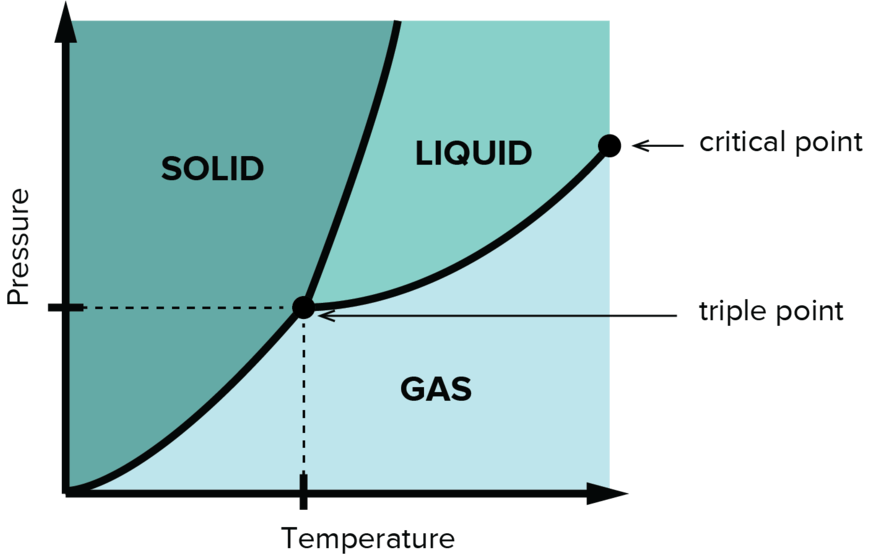
\includegraphics[height=3.6cm]{figs/2D-phase-diagram.png} \qquad 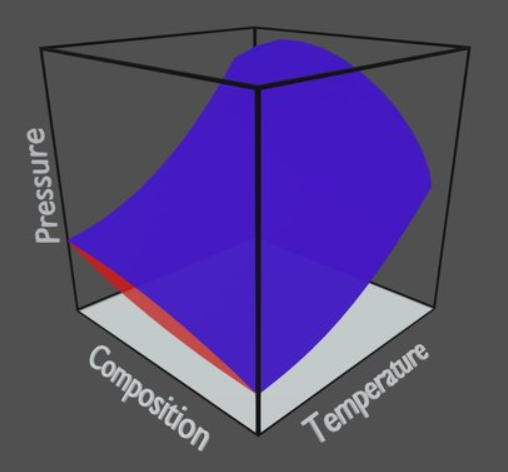
\includegraphics[height=3.6cm]{figs/3D-phase-diagram.png}

\end{frame}


\begin{frame}
    \frametitle{水的相图}
    \begin{columns}[c]
        \column{6.5cm}
        \\~
        \\        
        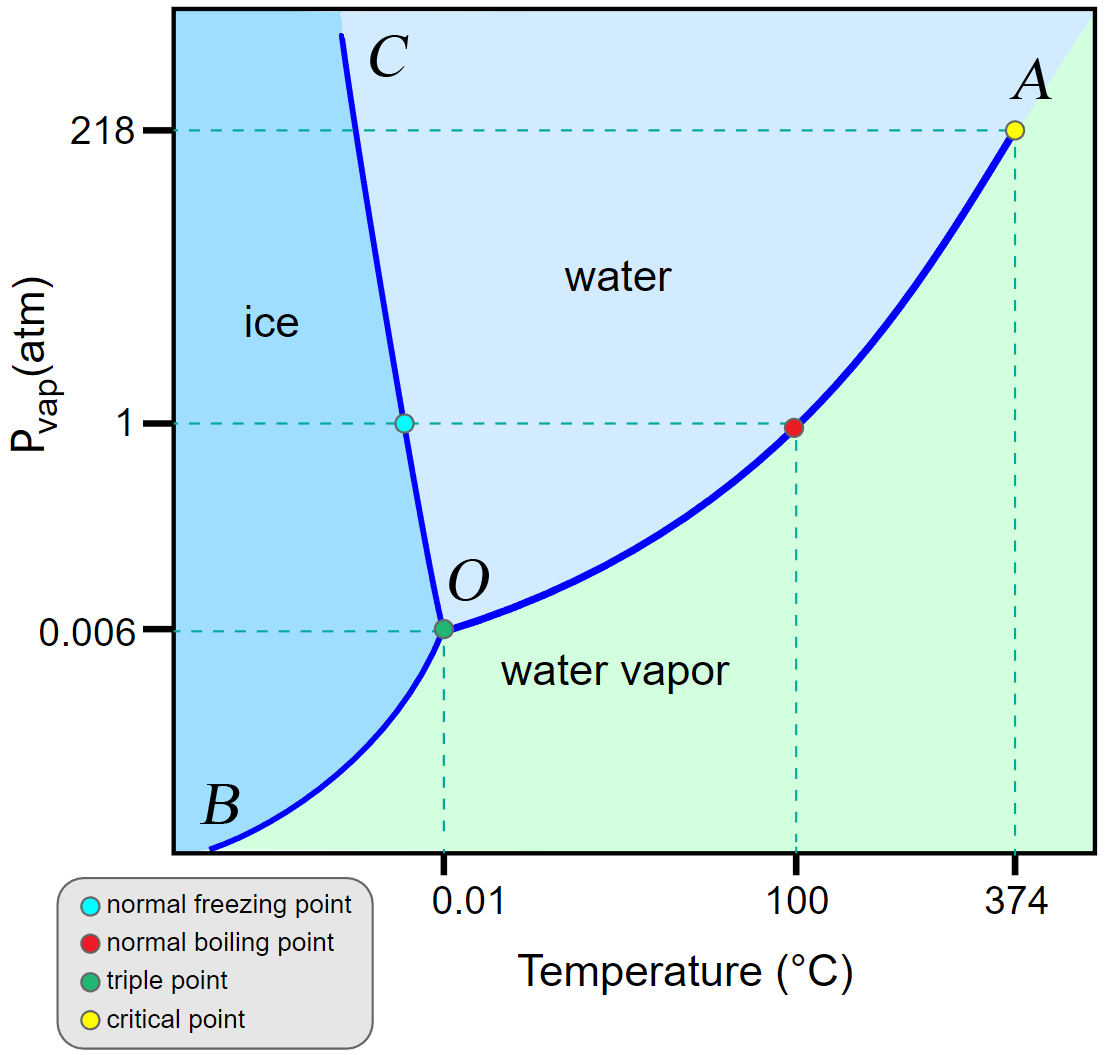
\includegraphics[width=6.5cm]{figs/phase-diagram-water.png}
        \column{7cm}
            \begin{itemize}
                \item[\bullet] 三个相区，每一相区$P=1,f=2$
                \item[\bullet] 三条线，每一条线上$P=2,f=1$
                \item[\bullet] OA气液平衡曲线(蒸汽压曲线)
                \item[\bullet] OB气固平衡曲线(升华曲线)
                \item[\bullet] OC液固平衡曲线(熔点线)
                \item[\bullet] O点：三相点，$P=3,f=0$ \\ 水的三相点$T$=273.16K，$p$=611Pa
            \end{itemize}
    \end{columns} 
\end{frame}